% supplement.tex -- Supplemental information for the HistoAtlas Patterns submission.
% Compile independently of main.tex.

\documentclass[11pt]{article}

\usepackage[T1]{fontenc}
\usepackage{lmodern}
\usepackage{amsmath,amssymb}
\usepackage{graphicx}
\usepackage{booktabs}
\usepackage{longtable}
\usepackage{siunitx}
\usepackage[table]{xcolor}
\usepackage[colorlinks=true,linkcolor=blue!60!black,citecolor=blue!60!black,
            urlcolor=blue!60!black]{hyperref}
\usepackage[top=1in,bottom=1in,left=1in,right=1in,letterpaper]{geometry}
\usepackage{caption}

\graphicspath{{../figures/}}
\sisetup{group-separator={,},group-minimum-digits=4}
\captionsetup{font=small,labelfont=bf}

\renewcommand{\thefigure}{S\arabic{figure}}
\renewcommand{\thetable}{S\arabic{table}}
\renewcommand{\figurename}{Figure}
\renewcommand{\tablename}{Table}

\title{\vspace{-2em}Supplemental information\\[0.4em]
\large HistoAtlas: an open, interpretable pan-cancer histomics resource linking
tissue morphology to molecular programs and clinical outcomes}
\author{Pierre-Antoine Bannier}
\date{}

\begin{document}
\maketitle

\noindent
This document (Document S1) contains Figures S1--S4 and Tables S1--S13. Tables marked \emph{machine-readable} are released in full with the
atlas rather than typeset here, because they contain between $10^3$ and $10^5$
rows; the file path given for each is relative to the root of the code
repository, and every one of them is also queryable through the web and
programmatic interfaces described in the main text. All statistics were produced
by the pipeline described in the main-text Methods; nothing in this document was
recomputed for presentation.

\tableofcontents
\clearpage

% =========================================================================
\section*{Supplementary Figures}
\addcontentsline{toc}{section}{Supplementary Figures}

\begin{figure}[htbp]
  \centering
  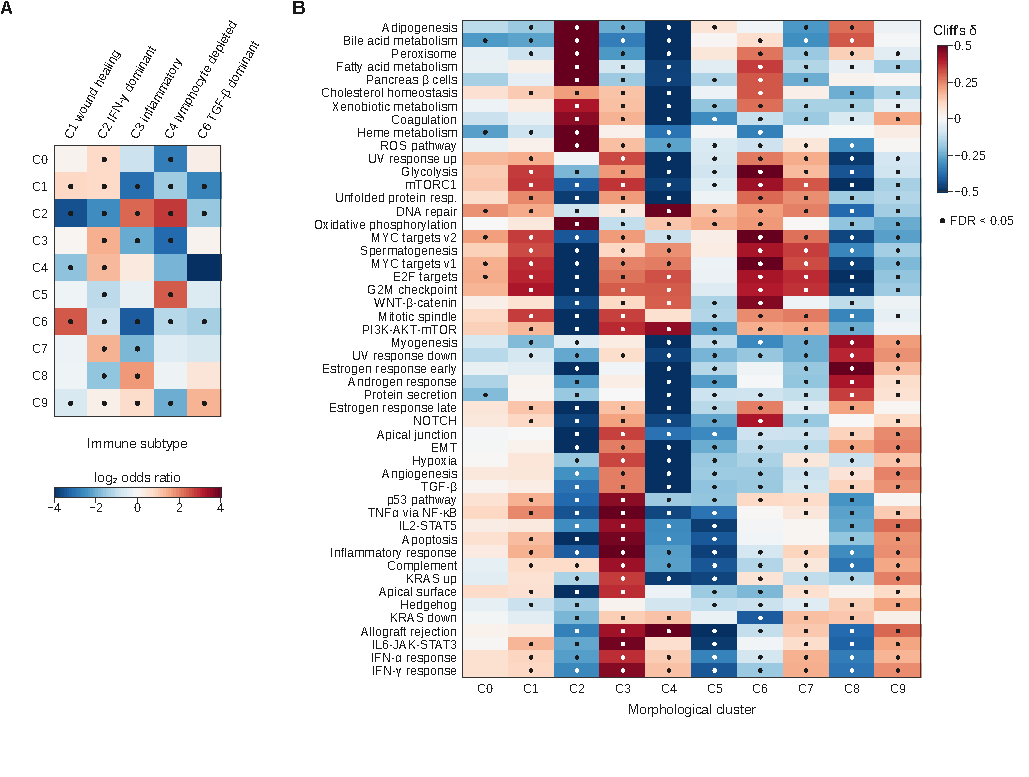
\includegraphics[width=\textwidth,height=0.62\textheight,keepaspectratio]{FigureS1.pdf}
  \caption{\textbf{Morphological clusters are enriched for distinct immune and
  pathway states.}
  (A)~Immune subtype enrichment per pan-cancer morphological cluster: $\log_2$
  odds ratio of each Thorsson immune subtype within the cluster versus the rest
  of the cohort (Fisher's exact test), clipped at $\pm 4$. Dots mark
  Benjamini--Hochberg adjusted $P < 0.05$.
  (B)~Hallmark pathway enrichment per cluster (Cliff's $\delta$ from Mann--Whitney
  $U$ tests, in-cluster versus out-of-cluster). Pathways are ordered by
  Ward-linkage clustering; dots mark Benjamini--Hochberg adjusted $P < 0.05$.
  These enrichments were computed after clustering and were not used to define
  the clusters, which were derived from the 38 histomic measurements alone.}
  \label{fig:s1}
\end{figure}

\begin{figure}[htbp]
  \centering
  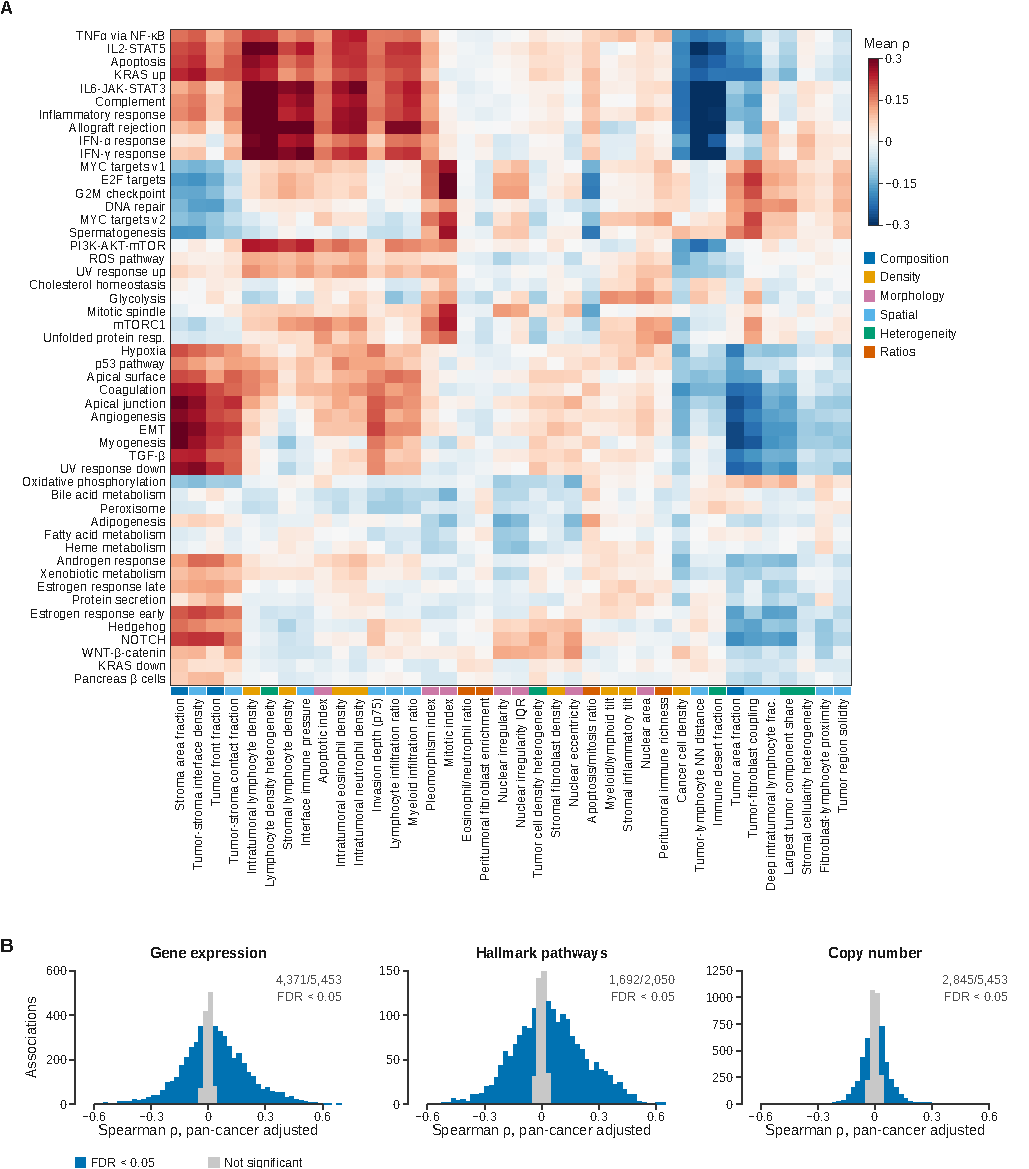
\includegraphics[width=\textwidth,height=0.62\textheight,keepaspectratio]{FigureS2.pdf}
  \caption{\textbf{Histomic measurements correspond systematically to Hallmark
  pathway activity.}
  (A)~Mean Spearman correlation across the 21 cancer types between each of the 38
  histomic measurements (columns) and each of the 50 MSigDB Hallmark pathway
  activity scores (rows), unadjusted model. Rows and columns are ordered by
  Ward-linkage clustering; the strip below the columns gives the measurement
  group. Immune-density measurements group with immune and inflammatory
  signatures; nuclear morphometry and mitotic index with cell-cycle and
  proliferation signatures; stromal and tumor--stroma interface measurements with
  epithelial--mesenchymal transition, angiogenesis and coagulation signatures.
  Color scale clipped at $\rho = \pm 0.3$.
  (B)~Pan-cancer covariate-adjusted Spearman coefficients by molecular data type,
  stacked histograms of significant (blue, false discovery rate below 0.05) and
  non-significant (gray) associations: gene expression, \num{4371} of \num{5453}
  significant (80\%); Hallmark pathways, \num{1692} of \num{2050} (83\%); copy
  number, \num{2845} of \num{5453} (52\%). $P$ values from the analytical
  $t$-approximation, Benjamini--Hochberg corrected within declared families.}
  \label{fig:s2}
\end{figure}

\begin{figure}[htbp]
  \centering
  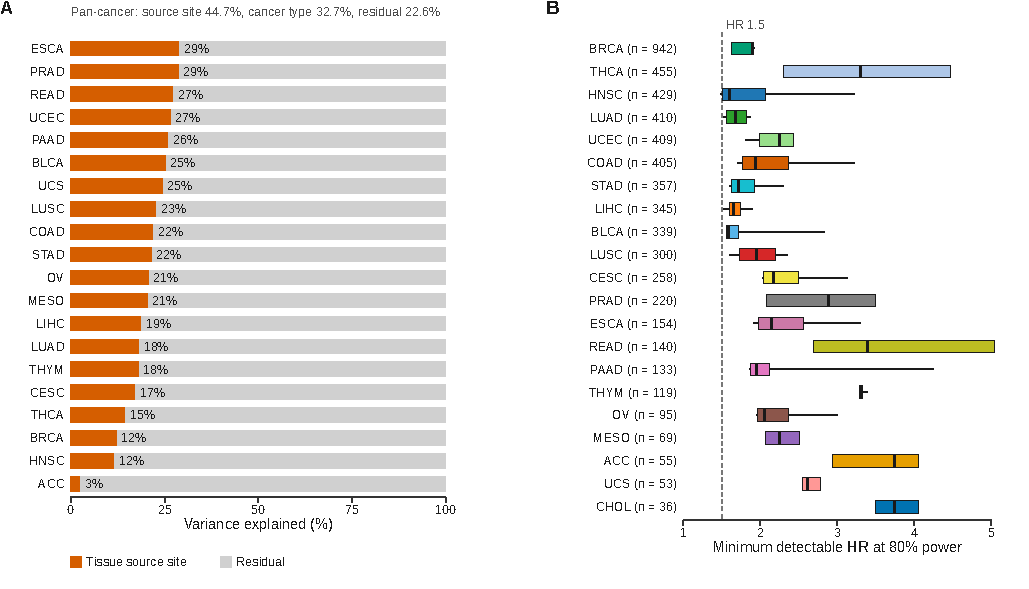
\includegraphics[width=\textwidth,height=0.62\textheight,keepaspectratio]{FigureS3.pdf}
  \caption{\textbf{Batch effects and statistical power.}
  (A)~Principal variance component analysis per cancer type: proportion of
  variance in the histomic measurements attributable to tissue source site
  (orange) and residual variance (gray), for the 20 cancer types with more than
  one source site. At pan-cancer level, 44.7\% of variance is attributed to source
  site, 32.7\% to cancer type and 22.6\% to residual; within cancer types, source
  site accounts for a median of 21.3\%. All per-cancer silhouette scores computed
  on source-site labels are negative ($-0.18$ to $-0.0004$), so slides do not
  segregate by source site in measurement space.
  (B)~Minimum detectable hazard ratio at 80\% power ($\alpha = 0.05$, two-sided)
  for harmful effects, by cancer type ordered by sample size ($n$, median patients
  per model). Boxes show the interquartile range across survival models, the bar
  the median and whiskers the 5th to 95th percentiles; dashed line, HR $= 1.5$.
  Breast carcinoma can detect HR $\geq 1.62$; cholangiocarcinoma ($n = 36$)
  requires HR $\geq 3.75$. Power, not absence of effect, explains why \num{4846}
  of \num{5623} survival associations carry an \emph{insufficient} evidence
  badge.}
  \label{fig:s3}
\end{figure}

\begin{figure}[htbp]
  \centering
  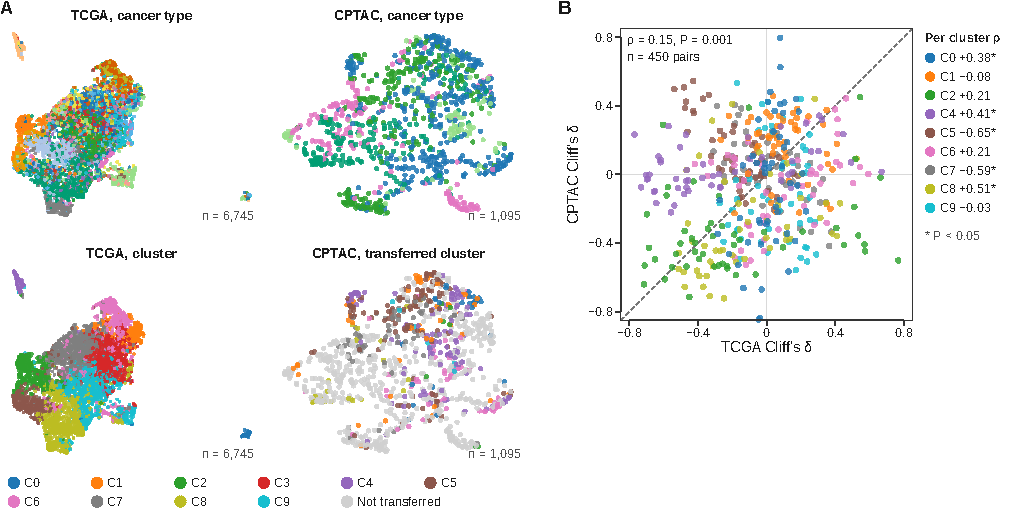
\includegraphics[width=\textwidth,height=0.62\textheight,keepaspectratio]{FigureS4.pdf}
  \caption{\textbf{Hard cluster labels transfer only partially to an independent
  cohort.}
  (A)~UMAP embeddings of TCGA ($n = \num{6745}$ slides, left) and CPTAC
  ($n = \num{1095}$ slides, right; a separate embedding computed on CPTAC),
  colored by cancer type (top; colors as in Figure 1C, HNSCC as HNSC) and by
  pan-cancer morphological cluster (bottom). CPTAC cluster labels were assigned by
  nearest-centroid prediction from the $K$-means model fitted on TCGA without
  refitting; slides without a complete measurement vector received no label
  (gray).
  (B)~Per-cluster pathway enrichment (Cliff's $\delta$) computed independently in
  TCGA (horizontal axis) and CPTAC (vertical axis) for 450 matched
  cluster--pathway pairs (no CPTAC slide was assigned to C3); dashed line,
  identity. Overall Spearman $\rho = 0.15$, $P = 1.4 \times 10^{-3}$. The list
  gives the per-cluster Spearman coefficient over 50 pathways; asterisks mark
  $P < 0.05$. Three clusters transfer positively ($\rho = 0.38$ to $0.51$) and two
  invert ($\rho = -0.59$ and $-0.65$). This result is why the main text treats the
  named measurements and the continuous programs, rather than the discrete
  clusters, as the portable products of the atlas.}
  \label{fig:s4}
\end{figure}

\clearpage
% =========================================================================
\section*{Supplementary Tables}
\addcontentsline{toc}{section}{Supplementary Tables}

% ---------------------------------------------------------------- S1
\begin{table}[htbp]
\centering
\caption{\textbf{Composition of the TCGA discovery cohort.} Diagnostic whole-slide
images after quality control, and the patients they come from. All slides enter
the descriptive analyses; statistical associations use one representative slide
per patient.}
\label{tab:s1}
\small
\begin{tabular}{llrr}
\toprule
Code & Cancer type & Slides & Patients \\
\midrule
BRCA & Breast invasive carcinoma & \num{1037} & \num{973} \\
LUAD & Lung adenocarcinoma & \num{511} & \num{448} \\
THCA & Thyroid carcinoma & \num{473} & \num{462} \\
HNSC & Head and neck squamous cell carcinoma & \num{471} & \num{449} \\
UCEC & Uterine corpus endometrial carcinoma & \num{459} & \num{421} \\
COAD & Colon adenocarcinoma & \num{441} & \num{433} \\
BLCA & Bladder urothelial carcinoma & \num{417} & \num{350} \\
STAD & Stomach adenocarcinoma & \num{400} & \num{375} \\
LIHC & Liver hepatocellular carcinoma & \num{365} & \num{357} \\
LUSC & Lung squamous cell carcinoma & \num{357} & \num{340} \\
PRAD & Prostate adenocarcinoma & \num{353} & \num{319} \\
CESC & Cervical squamous cell carcinoma & \num{279} & \num{269} \\
ACC & Adrenocortical carcinoma & \num{227} & \num{56} \\
THYM & Thymoma & \num{180} & \num{121} \\
ESCA & Esophageal carcinoma & \num{158} & \num{156} \\
READ & Rectum adenocarcinoma & \num{157} & \num{156} \\
PAAD & Pancreatic adenocarcinoma & \num{146} & \num{135} \\
OV & Ovarian serous cystadenocarcinoma & \num{107} & \num{106} \\
UCS & Uterine carcinosarcoma & \num{87} & \num{53} \\
MESO & Mesothelioma & \num{82} & \num{71} \\
CHOL & Cholangiocarcinoma & \num{38} & \num{38} \\
\midrule
\multicolumn{2}{l}{\textbf{Total (21 cancer types)}} & \textbf{\num{6745}} & \textbf{\num{6088}} \\
\bottomrule
\end{tabular}
\end{table}

% ---------------------------------------------------------------- S2
\begin{table}[htbp]
\centering
\caption{\textbf{TCGA cancer types excluded from the atlas.} All twelve were
excluded because their dominant cell morphologies fall outside the training
domain of the cell detection model, which was developed on epithelial and
squamous tissue. Exclusion was decided from the model's documented training
composition, before any downstream analysis.}
\label{tab:s2}
\small
\begin{tabular}{lll}
\toprule
Code & Cancer type & Dominant morphology outside training domain \\
\midrule
DLBC & Diffuse large B-cell lymphoma & Lymphoid cells \\
LAML & Acute myeloid leukemia & Myeloid blasts \\
GBM  & Glioblastoma multiforme & Glial cells \\
LGG  & Brain lower-grade glioma & Glial cells \\
SKCM & Skin cutaneous melanoma & Melanocytes \\
UVM  & Uveal melanoma & Melanocytes \\
SARC & Sarcoma & Mesenchymal cells \\
PCPG & Pheochromocytoma and paraganglioma & Neuroendocrine cells \\
KIRC & Kidney renal clear cell carcinoma & Renal tubular cells \\
KIRP & Kidney renal papillary cell carcinoma & Renal tubular cells \\
KICH & Kidney chromophobe & Renal tubular cells \\
TGCT & Testicular germ cell tumors & Germ cells \\
\bottomrule
\end{tabular}
\par\vspace{0.4em}
\parbox{0.92\textwidth}{\footnotesize Twenty-one of the 33 TCGA projects are
included (Table~S1) and these twelve are excluded. Of the 21
included types, 8 (LUAD, LUSC, BRCA, COAD, BLCA, OV, PAAD, MESO) are represented
in the cell model's training data and 13 were processed out of distribution;
per-cancer tissue--cell discordance rates and the resulting caveats are reported
in the main-text Methods.}
\end{table}

% ---------------------------------------------------------------- S3
\begin{table}[htbp]
\centering
\caption{\textbf{Definitions of the 38 histomic measurements.} Machine-readable.
Each row gives the measurement name, short and long descriptions, compartment,
unit, computation strategy, and both category assignments (the six-way
presentation grouping used in the main text and Figure~1, and the five-way
grouping stored in the atlas metadata). The two schemes partition the identical
38 measurements and no measurement differs between them.}
\label{tab:s3}
\small
\begin{tabular}{ll}
\toprule
Presentation category (main text, Figure 1) & $n$ \\
\midrule
Tissue composition & 3 \\
Cell densities & 8 \\
Nuclear morphology and kinetics & 7 \\
Spatial organization & 11 \\
Spatial heterogeneity & 5 \\
Cell-type ratios & 4 \\
\midrule
Atlas metadata category & $n$ \\
\midrule
Composition & 3 \\
Density & 6 \\
Morphology & 8 \\
Spatial & 18 \\
Heterogeneity & 3 \\
\bottomrule
\end{tabular}
\par\vspace{0.4em}
\parbox{0.92\textwidth}{\footnotesize Full definitions:
\texttt{histoatlas/config/feature\_metadata.py}; served by the
\texttt{list\_features} tool and at \url{https://histoatlas.com}.}
\end{table}

% ---------------------------------------------------------------- S4
\begin{table}[htbp]
\centering
\caption{\textbf{Curated molecular target panel.} Machine-readable. The 133
curated genes assessed for both expression and copy number, drawn from OncoKB
and the COSMIC Cancer Gene Census, together with immune checkpoint targets and
epithelial--mesenchymal transition and stemness markers; the 50 MSigDB Hallmark
gene sets, all used in the per-cancer correlation analysis; and
the 6 CIBERSORT immune cell fraction scores.
File: \texttt{histoatlas/config/molecular\_targets.py}.}
\label{tab:s4}
\end{table}

% ---------------------------------------------------------------- S5
\begin{table}[htbp]
\centering
\caption{\textbf{Benjamini--Hochberg correction family definitions.}
Machine-readable. One row per correction family, giving the family identifier,
the analysis type, the grouping keys, the number of tests in the family, and the
number significant at a false discovery rate below 0.05. Survival families are
defined per cancer type $\times$ endpoint $\times$ model (149 families);
correlation families per cancer type $\times$ molecular data type $\times$ model
(150 families). Every adjusted $P$ value in the atlas stores its family
identifier and family size, so any reported result can be re-derived.
Files: \texttt{correction\_family\_id} and \texttt{n\_tests\_in\_family} columns
of \texttt{survival\_associations.parquet} and
\texttt{feature\_correlations.parquet}.}
\label{tab:s5}
\end{table}

% ---------------------------------------------------------------- S6
\begin{table}[htbp]
\centering
\caption{\textbf{Complete-case sample sizes and covariate missingness.}
Machine-readable. Per cancer type and endpoint: total patients, events,
complete-case sample size, percentage dropped, per-covariate missing fractions
for age, sex and pathologic stage, whether multiple imputation was used, the
number of imputations, and the fraction of missing information.
Files: \texttt{n\_complete\_case}, \texttt{pct\_dropped},
\texttt{missing\_frac\_*}, \texttt{imputation\_used}, \texttt{n\_imputations} and
\texttt{fmi} columns of \texttt{survival\_associations.parquet}.}
\label{tab:s6}
\end{table}

% ---------------------------------------------------------------- S7
\begin{table}[htbp]
\centering
\caption{\textbf{Restricted mean survival time horizons and
proportional-hazards violation prevalence.} Machine-readable. Per cancer type:
the restricted mean survival time horizon in days and its justification, and the
proportion of fitted Cox models flagged pass, warn or fail on the Schoenfeld
residual test. Across all \num{5623} fitted models, \num{5283} passed
($P \geq 0.05$), 270 warned ($0.01 \leq P < 0.05$) and 70 failed ($P < 0.01$);
warned and failed models have their hazard ratios, confidence intervals and
$P$ values invalidated before correction.
Files: \texttt{rmst\_horizon\_days} and \texttt{ph\_flag} columns of
\texttt{survival\_associations.parquet}.}
\label{tab:s7}
\end{table}

% ---------------------------------------------------------------- S8
\begin{table}[htbp]
\centering
\caption{\textbf{Tests performed and significant results, by analysis type.}
Survival counts are Cox models; \emph{valid} excludes models whose
proportional-hazards assumption was violated. Significance is
Benjamini--Hochberg adjusted $P < 0.05$ within the declared families.}
\label{tab:s8}
\small
\begin{tabular}{llrrr}
\toprule
Analysis & Stratum & Tests & Valid & Significant \\
\midrule
Survival & Overall survival, unadjusted & 759 & 723 & 60 \\
Survival & Overall survival, adjusted & 721 & 691 & 21 \\
Survival & Progression-free survival, unadjusted & 836 & 770 & 77 \\
Survival & Progression-free survival, adjusted & 760 & 705 & 23 \\
Survival & Disease-specific survival, unadjusted & 722 & 671 & 53 \\
Survival & Disease-specific survival, adjusted & 648 & 614 & 12 \\
Survival & Disease-free survival, unadjusted & 608 & 569 & 12 \\
Survival & Disease-free survival, adjusted & 569 & 540 & 2 \\
\midrule
\multicolumn{2}{l}{\textbf{Survival total}} & \textbf{\num{5623}} & \textbf{\num{5283}} & \textbf{260} \\
\midrule
Correlation & Expression, unadjusted & \num{117436} & \num{117436} & \num{28182} \\
Correlation & Expression, adjusted & \num{85649} & \num{85649} & \num{22466} \\
Correlation & Pathway activity, unadjusted & \num{42150} & \num{42150} & \num{12397} \\
Correlation & Pathway activity, adjusted & \num{30200} & \num{30200} & \num{9591} \\
Correlation & Copy number, unadjusted & \num{117439} & \num{117439} & \num{6682} \\
Correlation & Copy number, adjusted & \num{85652} & \num{85652} & \num{6027} \\
Correlation & Immune scores, unadjusted & \num{5253} & \num{5253} & \num{1983} \\
Correlation & Immune scores, adjusted & \num{3859} & \num{3859} & \num{1592} \\
\midrule
\multicolumn{2}{l}{\textbf{Correlation total}} & \textbf{\num{487638}} & \textbf{\num{487638}} & \textbf{\num{88920}} \\
\bottomrule
\end{tabular}
\end{table}

% ---------------------------------------------------------------- S9
\begin{table}[htbp]
\centering
\caption{\textbf{CPTAC validation cohort and measurement concordance.} A
measurement passes when the standardized mean difference between cohort medians,
scaled by the TCGA standard deviation, is at most 1.0. A cancer type passes when
more than 80\% of the 38 measurements pass ($\geq 31/38$). Overall
inter-measurement correlation geometry across the pooled cohorts:
Pearson $r = 0.836$ on 703 upper-triangle pairs,
$P = 6.1 \times 10^{-185}$ (prespecified criterion $r > 0.80$; passed).}
\label{tab:s9}
\small
\begin{tabular}{llrrrrl}
\toprule
TCGA & CPTAC & TCGA $n$ & CPTAC slides & CPTAC patients & Within 1 SD & Pass \\
\midrule
LUAD & LUAD  & 511  & 240 & 240 & 34/38 (89.5\%) & yes \\
PAAD & PAAD  & 146  & 175 & 175 & 34/38 (89.5\%) & yes \\
HNSC & HNSCC & 471  & 390 & 112 & 32/38 (84.2\%) & yes \\
BRCA & BRCA  & \num{1037} & 198 & 198 & 31/38 (81.6\%) & yes \\
UCEC & UCEC  & 459  & 92  & 92  & 30/38 (78.9\%) & no \\
\midrule
\multicolumn{2}{l}{\textbf{Total}} & & \textbf{\num{1095}} & \textbf{817} & \textbf{4/5 pass} & \\
\bottomrule
\end{tabular}
\par\vspace{0.4em}
\parbox{0.94\textwidth}{\footnotesize Median tumor nuclear irregularity fails in
all five pairs (standardized mean difference 1.65 to 2.34, largest in lung
adenocarcinoma) and is flagged in the atlas as protocol-sensitive. The
endometrial carcinoma failure is driven by tissue-composition shifts in the
smallest cohort ($n = 92$ versus $n = 459$ in TCGA): stroma area fraction
(1.44 SD lower), tumor area fraction (1.25 SD higher), stromal fibroblast
density (1.29 SD lower) and tumor--stroma contact fraction (1.09 SD lower).}
\end{table}

% ---------------------------------------------------------------- S10
\begin{table}[htbp]
\centering
\caption{\textbf{Histomic program associations with protein abundance in
CPTAC.} Machine-readable, \num{2220} program--protein pairs across four cancer
types with proteomic profiles; 12.6\% significant at $P < 0.05$. Strongest
associations per program are given below.
File: \texttt{data/paper/histomic\_programs/program\_protein\_correlations.parquet}.}
\label{tab:s10}
\small
\begin{tabular}{llll}
\toprule
Program & Interpretation & Top protein correlates (Spearman $\rho$) \\
\midrule
P1 & Immune infiltration & CXCL9 (0.85), CD79A (0.82), CD3E (0.78) \\
P2 & Stromal architecture & ZEB1 (0.72), FN1 (0.71) \\
P3 & Nuclear atypia and proliferation & FGFR3 ($-0.70$), BRCA1 ($-0.64$) \\
P4 & Tumor density & --- \\
P5 & Myeloid inflammation & --- \\
P6 & Fibroblast biology & --- \\
\bottomrule
\end{tabular}
\end{table}

% ---------------------------------------------------------------- S11
\begin{table}[htbp]
\centering
\caption{\textbf{Benjamini--Hochberg versus Benjamini--Yekutieli correction.}
The Benjamini--Yekutieli procedure controls the false discovery rate under
arbitrary dependence among tests and is therefore more conservative. For this
comparison all tests of a given analysis type were pooled into a single
correction family, which is why the survival denominator (272) differs from the
260 obtained under the production 149-family design reported in the main text.}
\label{tab:s11}
\small
\begin{tabular}{lrrr}
\toprule
Analysis & Benjamini--Hochberg & Benjamini--Yekutieli & Retention \\
\midrule
Molecular correlations & \num{88920} & \num{60576} & 68.1\% \\
Survival associations & 272 & 147 & 54.0\% \\
\bottomrule
\end{tabular}
\end{table}

% ---------------------------------------------------------------- S12
\begin{table}[htbp]
\centering
\caption{\textbf{Sensitivity of leading correlations to molecular subtype
adjustment.} For each cancer type, the top 20 measurement--gene correlations were
recomputed with molecular subtype as an additional covariate. Attenuation is the
relative reduction in the median absolute Spearman coefficient.}
\label{tab:s12}
\small
\begin{tabular}{llrrrr}
\toprule
Cancer type & Subtype variable & Pairs & Median $|\rho|$ & Adjusted & Attenuation \\
\midrule
BRCA & PAM50 & 20 & 0.584 & 0.558 & 4.3\% \\
UCEC & Molecular class & 20 & 0.406 & 0.381 & 6.2\% \\
PAAD & Immune subtype (C1--C6) & 20 & 0.375 & 0.269 & 28.1\% \\
LUAD & \textit{EGFR}/\textit{KRAS} driver & 20 & 0.579 & --- & not evaluable \\
\bottomrule
\end{tabular}
\par\vspace{0.4em}
\parbox{0.94\textwidth}{\footnotesize The lung adenocarcinoma stratification was
uninformative because neither \textit{EGFR} nor \textit{KRAS} mutation was
prevalent enough in this cohort to form contrasting groups, leaving a single
category. Pancreatic adenocarcinoma shows substantially stronger subtype
confounding than breast or endometrial carcinoma; correlations in that cancer
type should be interpreted with subtype adjustment.}
\end{table}

% ---------------------------------------------------------------- S13
\begin{table}[htbp]
\centering
\caption{\textbf{Sensitivity of survival associations to leukocyte-fraction
adjustment.} The 10 leading survival measurements were refitted with leukocyte
fraction as an additional covariate, to test whether their prognostic signal is
a surrogate for immune content. It is not: slightly more associations reach
significance after adjustment. Machine-readable per-model results:
\texttt{data/paper/sensitivity/purity\_adjusted\_survival.parquet}
(358 fitted models).}
\label{tab:s13}
\small
\begin{tabular}{lrr}
\toprule
Model & Significant ($P < 0.05$) & Retention \\
\midrule
Base (clinical covariates) & 25/179 & --- \\
Leukocyte-fraction adjusted & 28/179 & 112\% \\
\bottomrule
\end{tabular}
\end{table}

\end{document}
